	\chapter{Object Detection}
	
	\label{sec:object_detection}
	
	\begin{center}
		\textbf{ How can a detection model represent wire frame objects?}
	\end{center}
	
	
	Object detection has been an intensively studied area within computer vision. Reaching back to \todoref{first object detection}, the machine based determination of what kind of objects we see where in the image has always been in the interest of academia and industry.
	
	On an abstract level the problem of object detection can be described by two individual tasks: Classification and Localization. While Classification deals with the question of what kind of object is displayed in the image, Localization is concerned with finding the position of objects. Hence, the output of a object detection system is usually a set of areas within the image and a corresponding class label:
	
	$$
	\begin{matrix}
	A_1, C_1\\
	..
	\end{matrix} = f(I)
	$$
	where $A_n$ describes an area, $C_1$ a class label, $I$ the image and $f(..)$ object detection.
	\todo{Image of pipeline}
	%Pipeline
	Images are high dimensional signals that can contain a lot of information which is not relevant for the task. As the performance of most machine learning models decreases when the feature space becomes too large (curse of dimensionality), most computer vision pipelines consists of two stages:
	\begin{enumerate}
		\item The feature extraction stage extracts task relevant information from the image and infers an internal, lower dimensional representation.
		\item The classification/localization stage receives this representation and produces the final output, which can be class probabilities and bounding box coordinates.
	\end{enumerate}  

	\section{Feature Extraction}
	
	In the first stage task/domain relevant properties of the input image are extracted to simplify the detection problem for later stages. Over the time different feature extractors also called filters evolved.
	
	\cite{Viola2004} use simple filters inspired by Haar-basis functions for human face detection. \cite{Dalal} and \cite{Lowe2004} compute a local (normalized) histogram of gradients for object detection. These approaches can be summarized as engineered feature extractors, as the filters are manually designed by incorporating task and domain specific knowledge. \todo{describe some pipelines and advantages}
	
	In recent years \acp{CNN} emerged from deep learning research and became a popular feature extractor. \acp{CNN} can be seen as small neural networks that are applied locally on image patches at various locations. In contrast to manually designed methods, \acp{CNN} can be learned task specific via back-propagation.
	
	With $i,j$ as location, $y$ as output, $f$ as activation function, $W$ as filter weights, $X$ as input and $b$ as bias, the convolution operation can be expressed as follows:
	
	$$Y_{ij} = f(WX_{ij} + b)$$
	
	where the size of $W$ depends on the kernel size $k$ and the locations are usually chosen in sliding window manner with a certain step size $s$, also called strides.
	
	\acp{CNN} offer the advantage that they can be stacked on top of each other and therefore be combined in several layers to learn highly non-linear representations.
	\todoref{arg1} demonstrate a very efficient architecture in which only 3x3 kernels are used. That way early layers focus on fine grain details and basic features like edges and corners, while higher order layers combine these features to more complex shapes. 
	
	Various studies suggest that going deeper with convolutions increases representation strength yielding even better results. However, such high performance comes at a cost. As \acp{CNN} grow deeper inference time and memory usage increase as well.
	
	Next to the standard convolutional kernel several variations can be found in literature: Atrous/Dilated convolutions consist of a sparse kernel thereby increasing the receptive field of a filter without increasing complexity or number of computations \todoref{Atrous}. Deformable convolutions allow a kernel shape different from the standard symmetric kernel \todo{deformable cnn}.
	
	Different activation functions have emerged. $Tanh$ and sigmoid-activations produce naturally an output at a small range which simplifies the optimization. However, when the filter output falls unfavourably, the gradient with respect to the activation is almost zero leading to much longer training times. This issue gave rise to the family of rectified linear units (ReLU) which have been generalized in \todoref{..} to parametrized linear units (PReLU):
	
	$$
		f(x) = \begin{cases}
			x \quad \text{for } x \geq 0 \\
			\alpha x \quad \text{for } x < 0
		\end{cases}
	$$
	
	The issue of network initialization and "saturating" activations is also addressed in \cite{Ioffe2015}. With batch normalization the authors introduce a layer that normalises the data batch-wise and is fully differentiable. Including batch normalization after a convolutional layer leads to more stable and faster convergence. \todoref{arg1} show how using batch normalization cancels out the bias term.
		
	Using a convolutional layer followed by batch normalization and non-linear activation evolved to a standard in classification and object detection pipelines. It can be summarized in:
	
	\todo{doublecheck}
	$$
	Y_{ij} = f(\frac{WX_{ij}}{\sigma}+c)
	$$
	

	Various authors show how \acp{CNN}-based methods outperform methods with engineered feature extractors by far\todoref{Alexnet,}. \cite{Razavian}s experiments show how that this is not only because \acp{CNN}-features are trained on a specific task, but that  the learned representation is quite general and can be used in other vision tasks and methods.
	
	This has led to common practice to train feature extractors with a classification task on the Imagenet dataset with \todo{number} images and to use these weights to initialize networks for other tasks like object detection or segmentation. Popular feature extractors are summarized in \autoref{tab:cnn-extractors}.
	
	\begin{table}[htbp]
		\centering
		\caption{Popular Feature Extractors}
		\begin{tabular}{l|l|l|l}
			Name & Layers & Number of Weights &  \\ \hline
			VGGNet &  &  &  \\ \hline
			ResNet &  &  &  \\ \hline
			GoogLeNet &  &  &  \\ \hline
			MobilenetV2 &  &  &
		\end{tabular}
		\label{tab:cnn-extractors}
	\end{table}
	
	
	

	\section{Sampling}
	
	Without simplifying assumptions the total amount of objects in an image is not known at test time. Thus it is necessary to classify multiple regions within an image, to determine class labels and object locations. However, the amount of combinations between regions and objects that can appear in an image is infinite, while usually a large proportion of the image does not contain any object. Hence, which areas to sample within an image is a critical parameter regarding performance in accuracy and inference time.
	
	Commonly the areas to classify are limited bounding boxes that surround the object. However also other have been proposed..	
	
	
	
	\subsection{Sliding window}
	
	Sliding window based techniques sample the image by cropping regions of different sizes and aspect ratios across the image. Usually, the whole image is covered by moving the window from top left to bottom right. 
	
	This technique is applied in \todo{put examples}
	
	Sliding window techniques cover the whole input space and are easy to implement. However, the methods do a lot of superflous and redundant computations e.g. when most parts of the image are empty or certain regions are covered multiple times.
	
	\subsection{Attention Models}
	
	Attention based techniques are inspired by the human vision process \todoref{arg1}. The algorithm focusses on the important parts of the image and doesn't spend computations on less important parts. Multiple approaches exist to model the attention process.
	
	\citeauthor{Viola2004} use a cascaded of classifier that are evaluated in iterative fashion. Is a certain patch classified as background, its not further processed.
	
	Guido proposes a neural network to learn an attention model.
	
	X propose a recurrent neural network architecture to model the attention process.
	
	Fast-RCNN \cite{Ren} and Faster-RCNN \cite{Ren2015} formulate the attention process as regression problem and model it with a \acp{CNN} that proposes regions which possibly contain an object. The proposed regions are classified in a second step. 
	

	%			\paragraph{Scalable Object Detection using Deep Neural Networks\cite{Erhan}}
	%			\begin{itemize}
	%				\item[-] Generates number of bounding boxes as object candidates (class agnostic) and confidences for each box
	%				\item[-] For each Bounding Box a classifier is run e.g. DNN
	%				\item[-] Training: If the number of boxes k is larger than the number of objects b, only b boxes are matched while the confidence of the others is minimized
	%				\item[-] Assignment problem $$F_{match}(x,l) = \frac{1}{2}\sum_{i,j}x_{ij}||l_i - g_j||^2_2$$ where $x_ij$ is one if the ith prediction is assigned to the jth ground truth object
	%				\item[-] Confidence: 
	%				$$F_{conf}(x,c) = - \sum_{i,j}x_{ij}*\log(c_i)-\sum_{i}(1-\sum_{j}x_{ij})\log{1-c_j}$$
	%				\item[-] Speed up training by clustering (kmeans) of ground truth and using it as prior (prior matching)
	%				\item[-] Can be defined to output boxes only for a particular class by training the bounding boxes on that class
	%				\item[-] Number of parameters grows linearly with number of classes
	%				\item[-] Authors argue two step process (region proposal + classification) is better
	%				\item[-] Architecture based on AlexNet
	%				\item[-] Predicted boxes are merged using non-maxima surpression
	%				\item[-] One shot(50\%), +2scales (75\%)
	%				\item[-] OverFeat/ Selective Search are faster but much more expensive
	%			\end{itemize}
	
	\section{Object Model}
	
	In the last stage the extracted features are used to assign a class label to certain regions. Different approaches for this stage exist.
	
	The straight forward approach is to feed the features from all cropped regions into a classifier, and assign a certain class label. That way the object model is learned separated from the detection task. This concept can be found in \todo{examples} where support vector machines or neural networks are used.
	
	However, these methods prove to be sensitive towards part occlusions or large deformations. This gave raise to deformable part models where parts of the object are explicitly learned and detected.  \todo{describe springs}
	
	The deep learning approaches could significantly surpass the detection accuracy of the mentioned approaches without the concept of deformable part models. However, \todoref{cnns are dpms} shows experimentally that \acp{CNN} internally learn a similar representation.
	
	\cite{Viola2004}.

	\section{Regression Models}
	
	\iffalse
	\begin{figure}[hbtp]
		
		\centering
		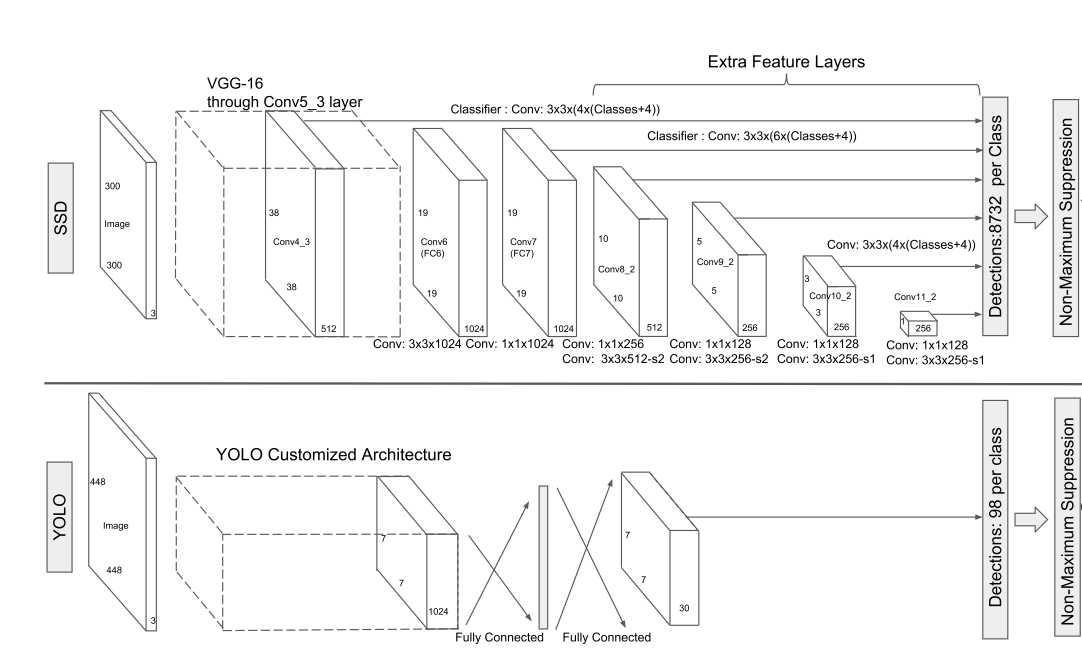
\includegraphics[width=\linewidth]{fig/architecture}
		\caption{Typical Architecture for One Stage Detectors}
		\label{fig:architecture}
		
	\end{figure}
	\fi
	Regression models incorporate all stages of object detection in one model and formulate the task as regression problem. Predictions are made for a predefined set of regions. The process is usually modelled with deep neural networks.
	
	\citeauthor{Redmon} were the first to publish such a method in \cite{Redmon}. The task is formulated by dividing the input image in a fixed grid and defining output nodes with softmax activation to predict $C$ class probabilities for each grid cell. Additional $5*B$ output nodes predict $B$ set of bounding box coordinates and $B$ object probabilities for each cell. This leads to a total number of $S*S*B*(4 + 1 + C)$ output nodes. 
	
	YoloV2, SSD  formulate the task by discretizing the output as a set of preparameterized bounding boxes. For each box class probabilities and bounding box offsets are predicted. In total this leads to $S*S*B*(4 + 1 + C)$ output nodes. 
	
	The models are trained by assigning a certain set of output nodes the "responsibility" to predict a certain object. That means only the output for these nodes is taken into account when calculating the loss for a certain sample and when updating the weights in the backward pass. This "matching strategy" is usually based on the intersection-over-union between ground truth and anchor box. \autoref{fig:anchors} illustrates the concept in the example of SSD.  
	
	\begin{figure}[hbtp]
		
		\centering
		\captionsetup{justification=raggedright,singlelinecheck=false}
		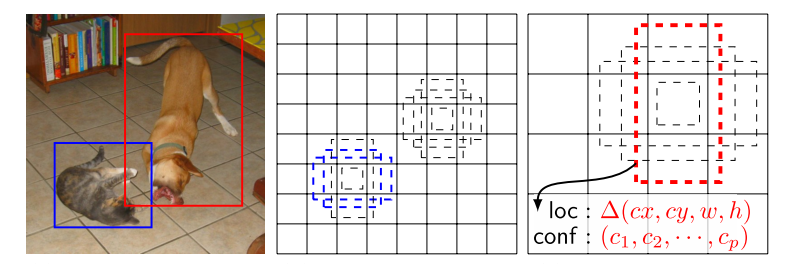
\includegraphics[width=0.8\linewidth]{fig/anchors}
		\caption{The anchor boxes are displayed as dashed lines. The ground truth label of the cat in blue is assigned to two anchor boxes. The output nodes predicting coordinate offset $\Delta(cx, cy, w,h)$ and class probabilities $c_1 .. c_p$ corresponding to these two boxes take part in the loss calculation \cite{Liu}.}
		\label{fig:anchors}
		
	\end{figure}
	
	Within this framework several approaches exist that either change the base network or modify layers in between: \cite{ChengchengNing2017} propose propose a more efficient non-max-suppression method as well as to include an inception module in the network architecture to reduce computation while keeping/increasing performance. \cite{Wu} uses \textit{SqueezeNet} as base network and a mixture between the ssd and yolo loss function as training goal. \cite{Xiang} investigates the receptive fields of SSD and tries to incorporate more context, especially on lower feature maps, to increase detection rate for small objects.\cite{Linb} applies the framework for vehicle detection. They use \textit{GoogLeNet} as base network (and investigate several others).\cite{TripathiSanDiego} apply a network very similar to YoloV2 and investigate 8bit quantization of the model to make it runnable on embedded devices.
	
	A common problem of one stage detectors is the imbalance between background and object samples. Most methods upweigh the positive samples and/or use hard negative mining. \cite{Lin} introduces the \textit{Focal Loss} which focuses on sparse positive samples by design.
	
	Each of the described group of methods has strengths and weaknesses. While shallow methods are typically quite fast they require a lot of manual effort and/or are not so accurate. Two-stage detectors on the other hand are quite accurate but their computational requirements are prohibitive for the hardware to be used in this thesis. One-stage detectors offer a compromise between detection accuracy and inference speed. In addition they can be trained end-to-end which requires only little manual engineering. However, the presented methods are still too slow for the hardware used in this thesis.




\todo{Elaborate, It should become clear why we use deep learning}


\section{Wire-frame objects}

\todo{Definition of a wireframe object}

The properties of wireframe object can be summarized in:
\begin{enumerate}
	\item It does not consist of complex shapes but only basic geometric shapes like corners, edges
	\item The object parts themselves are thin structures
	\item The object parts are sparse. The bounding box around the object is largely occupied by background
\end{enumerate}

\todoref{Wire detection}
\todoref{Method from last year, Other papers on drone racing}

\section{Hypothesis}

Several hypothesis are formulated and will be examined experimentally:
\begin{enumerate}
	\item \textbf{A \acp{CNN} should be able to learn the object detection task.}
	\item \textbf{For wireframe objects the deeper layers don't learn anything as the object consist of relatively simple shapes.}
	\item \textbf{The detection of fine grain structures is important.}
\end{enumerate}
\newpage
\section{Experiments}

\todo{Show how current methods perform on wire frame objects - performance over angle}
\todo{Reduce number of parameters and compare to big model}
\todo{What do the individual layers learn, where does it fail}
\todo{sensitivity analysis what triggers the network?}

\section{Conclusion}